% Pursuing Stacks (cotes 134-2 to 134-8): archive cote 134-6, site page 57 (PDF page 58), typescript page 375.
% typescript. Draft compared: ps5.tex:4196-4289.
% AI-transcribed by Claude Opus 5.5 (claude-opus-5-5, adaptive thinking, effort high), Message Batches API, batch ps3 (msgbatch_01XdFmuVVBAcgc7EFxdtCqsj), 2026-11-12; reviewed against both supplied scan halves; see CHECK_DECISIONS.tsv.
\scanpage{134-6/57}
\mspage{375}

where the \over{\unsure{vertical}}{horizontal} arrows \over{\unsure{ar}}{ar}e the canonical inclusion functors, and
\over{a}{A}ddinf(f) is the ``tautological'' extension of $f:B'\hand{\to} B$ to the infinitely
additive envelopes, defined computationally as
\margin{\tikz[baseline=(bi.base)]{\node[inner sep=3pt] (bi) {\ensuremath{b_i^{\prime}}};\draw[color=blue] (bi.center) ellipse (1.6em and 1.4em);}}
(2) \[ \over{a}{A}\mathrm{ddinf}(f)(L') \hand{\simeq} \deleted{\xout{\unsure{f_!^{ab}(L')}}} \hand{\bigoplus}_{i\hand{\in} I} \underline{Z}^{f(b_i\hand{'})} \]
for an object of Addinf(B') written canonically as
(3) \[ L' = \hand{\bigoplus}_{i\hand{\in} I} \underline{Z}^{(b_i\hand{'})} \quad . \]
Here, for an object b in a small category B, we denote by the more sugges%
% NOTE: the end of this line is cut by the right edge of the scan
-tive symbol $\underline{Z}^{(F)}$ the abelianization $\mathrm{Wh}_B(F)$ of an object F of $B^{\hand{\wedge}}$ , and
accordingly if F is an object b in B. The fact that (2) is equally an
expression for $f_{\hand{!}}^{ab}$ follows immediately from commutation of $f_{\hand{!}}^{ab}$ to small
direct sums, and from the canonical isomorphism
(4) \[ f_{\hand{!}}^{ab}(\underline{Z}^{F'}) \hand{\simeq} \underline{Z}^{(f_{\hand{!}}(F'))} \quad , \]
i.e. commutation up to canonical isomorphism of the diagram
(5) \diagram{\begin{tikzcd}
B'^{\hand{\wedge}} \ar[color=blue,r,"\mathrm{Wh}_{\hand{B'}}"] \ar[color=blue,d,"\hand{f_!}"'] \& B'^{\hand{\wedge}}_{ab} \ar[color=blue,d,"\hand{f_!^{ab}}"] \\
B^{\hand{\wedge}} \ar[color=blue,r,"\mathrm{Wh}_{\hand{B}}"] \& B^{\hand{\wedge}}_{ab}
\end{tikzcd}} ,
% NOTE: in (5) the horizontal and vertical arrows are drawn by hand
the verification of which is immediate. (For a generalization to sheaves
endowed with arbitrary ``algebraic structures'' and taking free objects,
see SGA 4 I 5.8.3.(p. 30).)

Of course, (1) and (2) imply that \xout{the} $f_{\hand{!}}^{ab}$ maps \xout{the} Add(B')
into Add(B), and induces the tautological extension Add(f) \xout{between} of
f to the additive envelop\xout{p}es. Thus (1) and (5) can be inserted in\hand{t}\over{o}{o} \hand{a}
be\deleted{a}\inserted{au}tiful commutative diagram (up to canonical isomorphisms)
\margin{\tikz[baseline=(cn.base)]{\node[inner sep=3pt] (cn) {\shortstack{Centrer\\et déployer}};\draw[color=blue] (cn.center) ellipse (4.4em and 2.5em);}}
\hand{(6)} \diagram{
% Hand-drawn arrows are marked blue; typed objects remain plain.
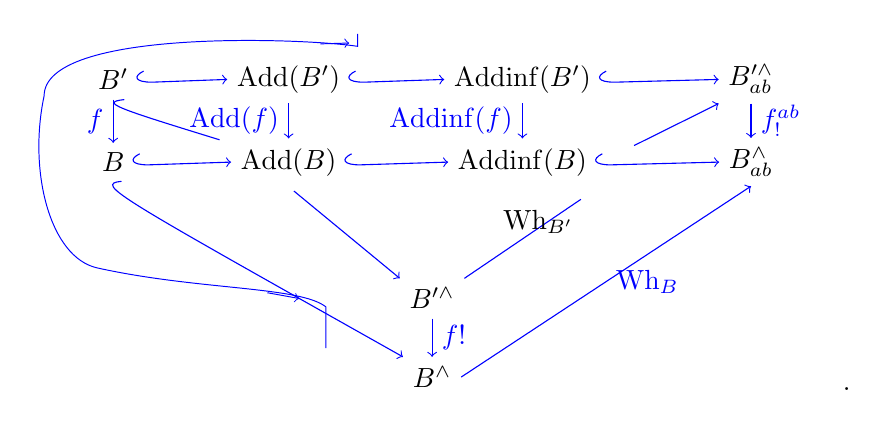
\begin{tikzpicture}[x=1.35cm,y=1.05cm,baseline=(bp.base)]
\node (bp) at (0,0) {\ensuremath{B'}};
\node (b) at (0,-1) {\ensuremath{B}};
\node (ap) at (1.65,0) {\ensuremath{\mathrm{Add}(B')}};
\node (a) at (1.65,-1) {\ensuremath{\mathrm{Add}(B)}};
\node (ip) at (3.85,0) {\ensuremath{\mathrm{Addinf}(B')}};
\node (i) at (3.85,-1) {\ensuremath{\mathrm{Addinf}(B)}};
\node (up) at (6,0) {\ensuremath{B'^{\hand{\wedge}}_{ab}}};
\node (u) at (6,-1) {\ensuremath{B^{\hand{\wedge}}_{ab}}};
\node (sp) at (3,-2.65) {\ensuremath{B'^{\hand{\wedge}}}};
\node (ss) at (3,-3.6) {\ensuremath{B^{\hand{\wedge}}}};
\foreach \s/\t in {bp/ap,ap/ip,ip/up,b/a,a/i,i/u}{
 \draw[color=blue,->] ([xshift=2pt,yshift=3pt]\s.east) .. controls ([xshift=-2pt,yshift=1pt]\s.east) and ([xshift=-1pt,yshift=-1pt]\s.east) .. ([xshift=5pt,yshift=-1pt]\s.east) -- (\t.west);
}
\draw[color=blue,->] (bp.south)--node[left]{\ensuremath{\hand{f}}}(b.north);
\draw[color=blue,->] (ap.south)--node[left]{\ensuremath{\hand{\mathrm{Add}(f)}}}(a.north);
\draw[color=blue,->] (ip.south)--node[left]{\ensuremath{\hand{\mathrm{Addinf}(f)}}}(i.north);
\draw[color=blue,->] (up.south)--node[right]{\ensuremath{\hand{f_!^{ab}}}}(u.north);
\draw[color=blue] ([xshift=4pt]bp.south) .. controls ([xshift=-5pt,yshift=-1pt]bp.south) and ([xshift=1pt,yshift=-3pt]bp.south) .. (1.0,-.73);
\draw[color=blue,->] (1.7,-1.35)--(sp.north west);
\draw[color=blue,->] ([xshift=3pt]b.south) .. controls ([xshift=-7pt,yshift=-1pt]b.south) and ([xshift=1pt,yshift=-5pt]b.south) .. (ss.north west);
\draw[color=blue,->] (sp.south)--node[right]{\ensuremath{\hand{f!}}}(ss.north);
\draw[color=blue] (sp.north east)--(4.4,-1.45);
\draw[color=blue,->] (4.9,-.80)--(up.south west);
\node at (4.0,-1.72) {\ensuremath{\hand{\mathrm{Wh}_{B'}}}};
\draw[color=blue,->] (ss.east)--node[right]{\ensuremath{\hand{\mathrm{Wh}_{B}}}}(u.south);
\draw[color=blue,line width=.35pt] (2.3,.55)--(2.3,.40) .. controls (1.8,.50) and (-.65,.62) .. (-.65,-.20) .. controls (-.8,-1.1) and (-.6,-2.15) .. (-.15,-2.28) .. controls (.8,-2.55) and (1.75,-2.5) .. (2.0,-2.75)--(2.0,-3.25);
\draw[color=blue,->,line width=.35pt] (1.95,.43)--(2.22,.44);
\draw[color=blue,->,line width=.35pt] (1.45,-2.58)--(1.75,-2.65);
\node at (6.9,-3.75) {.};
\end{tikzpicture}}
% Reviewed diagram(6): all arrows are hand-drawn; object names are typed. The two interrupted diagonals and the unattached outer pencil enclosure are preserved as drawn.

The formula (1) (or equivalently, (2)) can be viewed as giving a
computational description of the left derived functor \xout{Lf}
(7) \[ \mathrm{L}f_{\hand{!}}^{ab} : D^{\hand{-}}(B'^{\hand{\wedge}}_{ab}) \hand{\to} D^{\hand{-}}(B^{\hand{\wedge}}_{ab}). \]

\margin{57}

% Visual collation: both supplied image halves inspected; see CHECK_DECISIONS_134_7_8.tsv.
